\begin{figure*}[t]
    \centering
      \subfloat{
          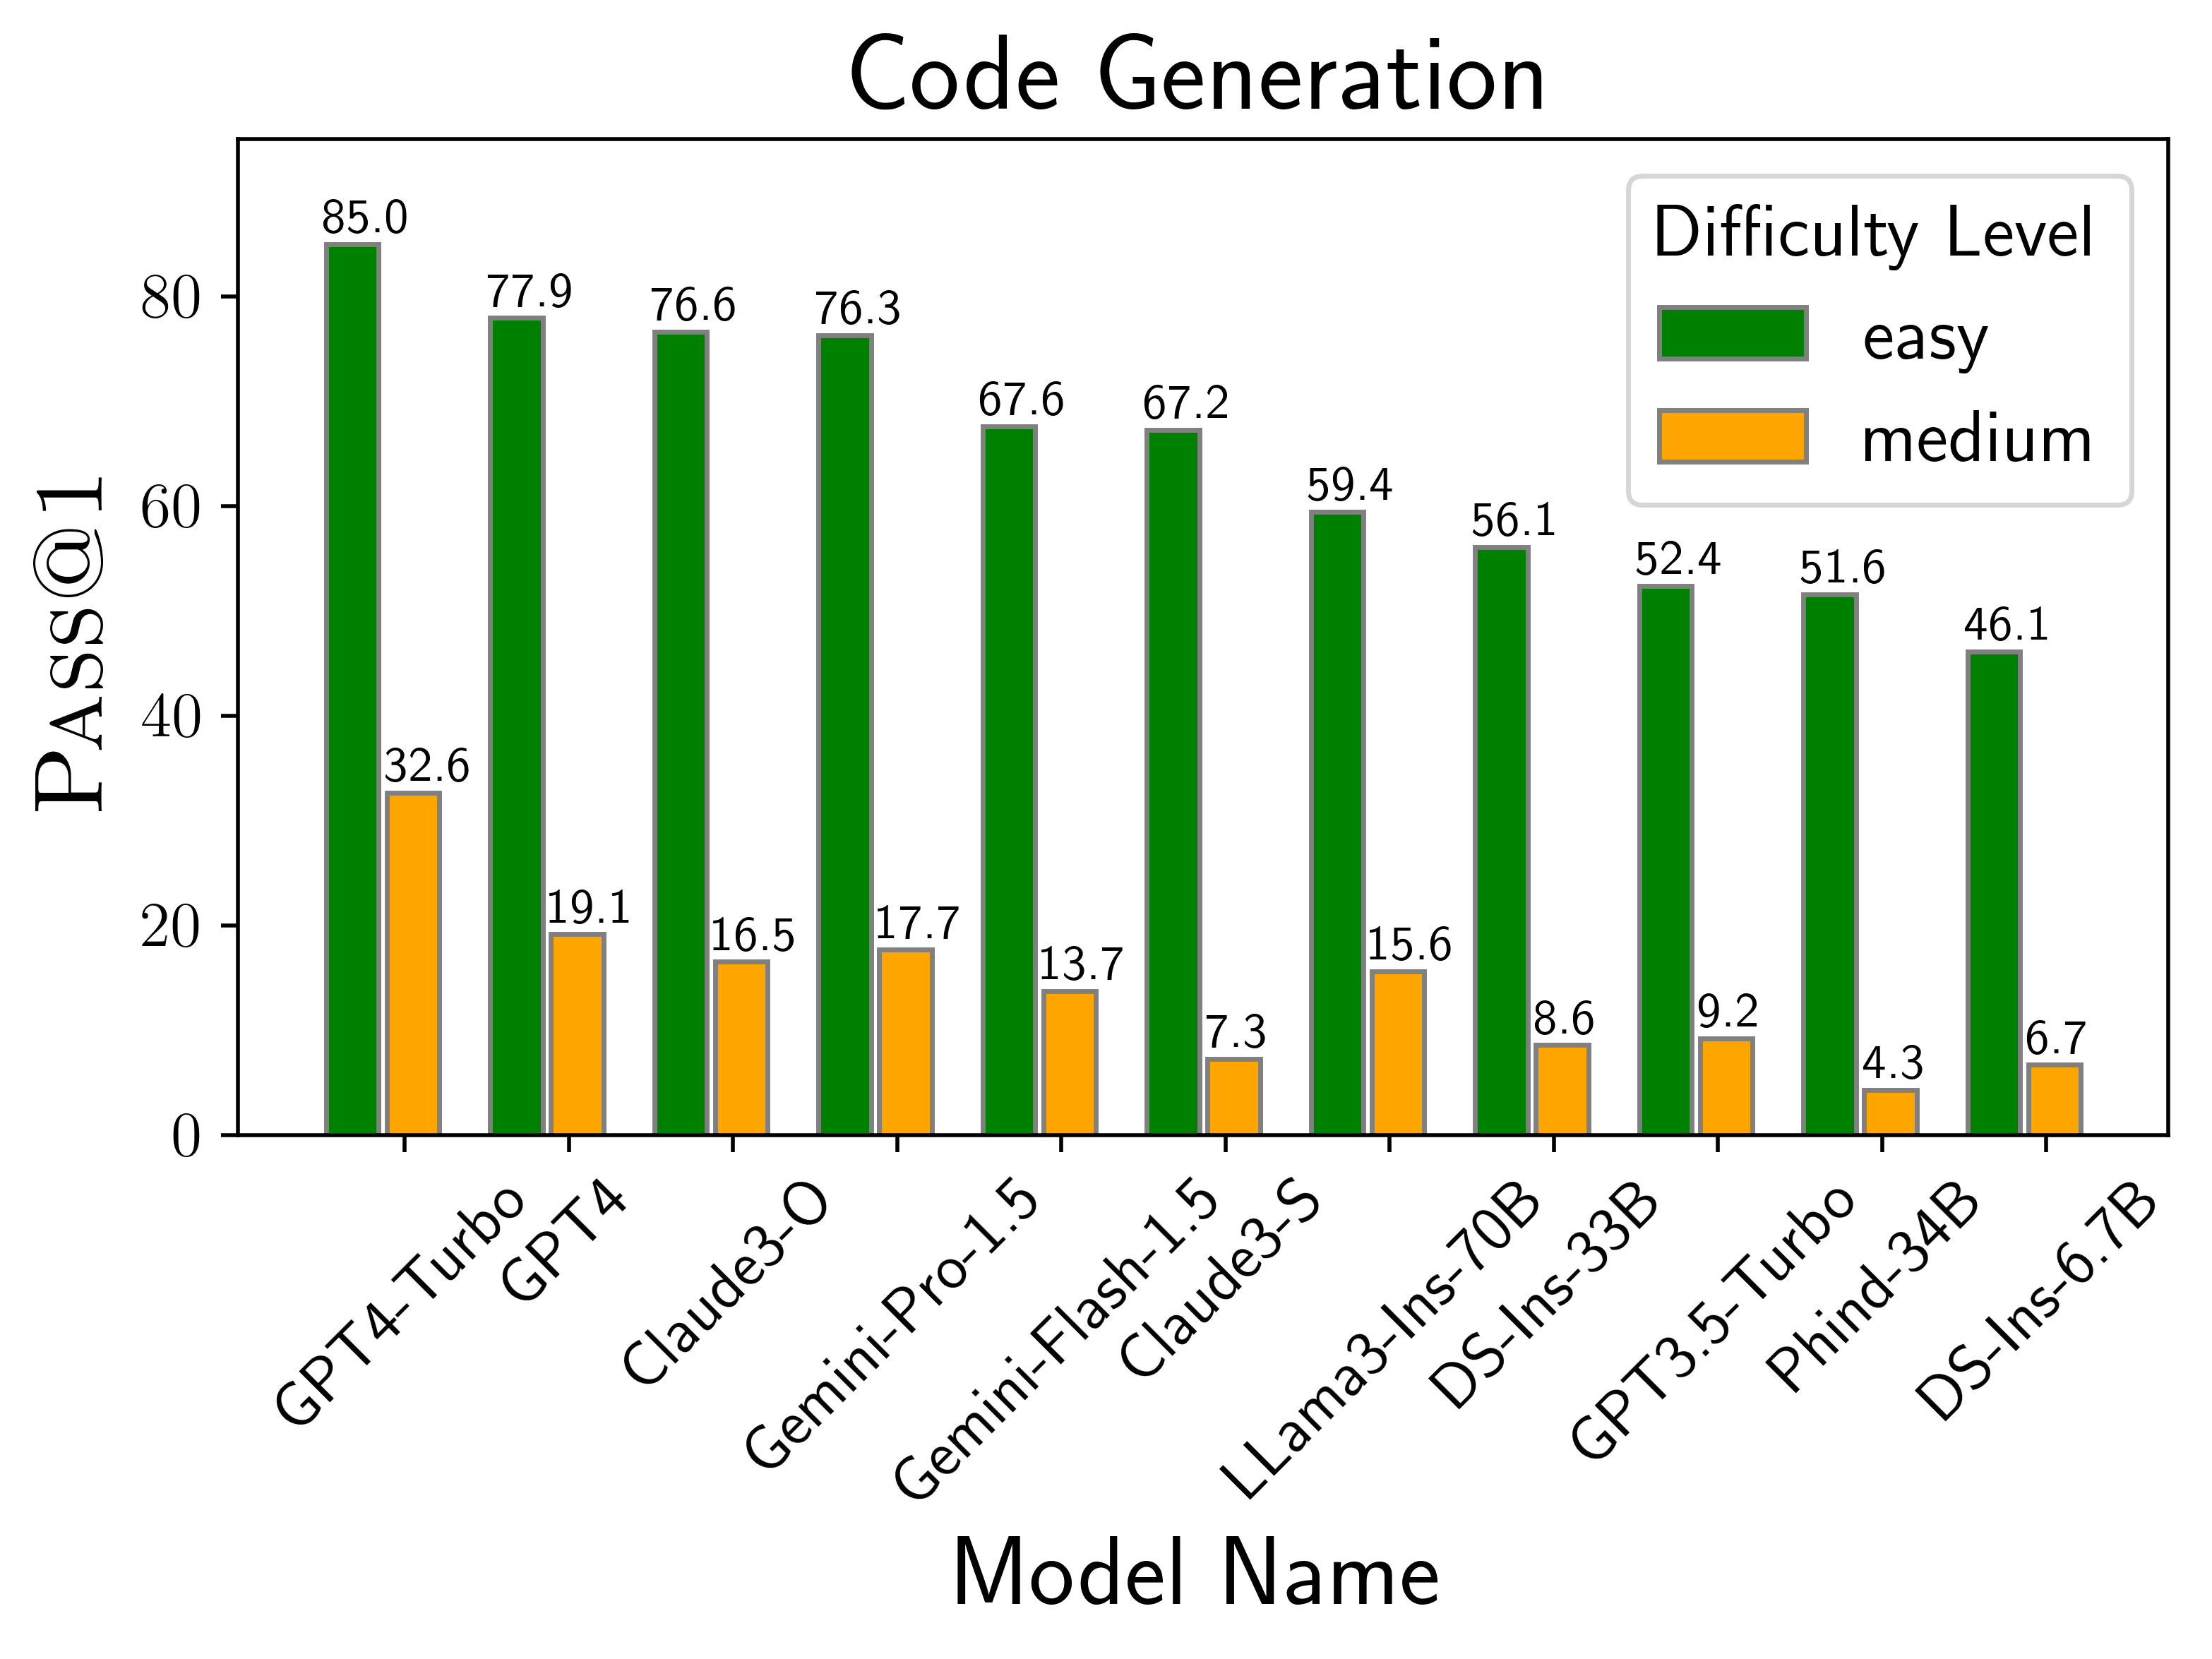
\includegraphics[width=0.48\linewidth]{figures/main_results/codegen_performance.png}}
      ~
      \subfloat{
          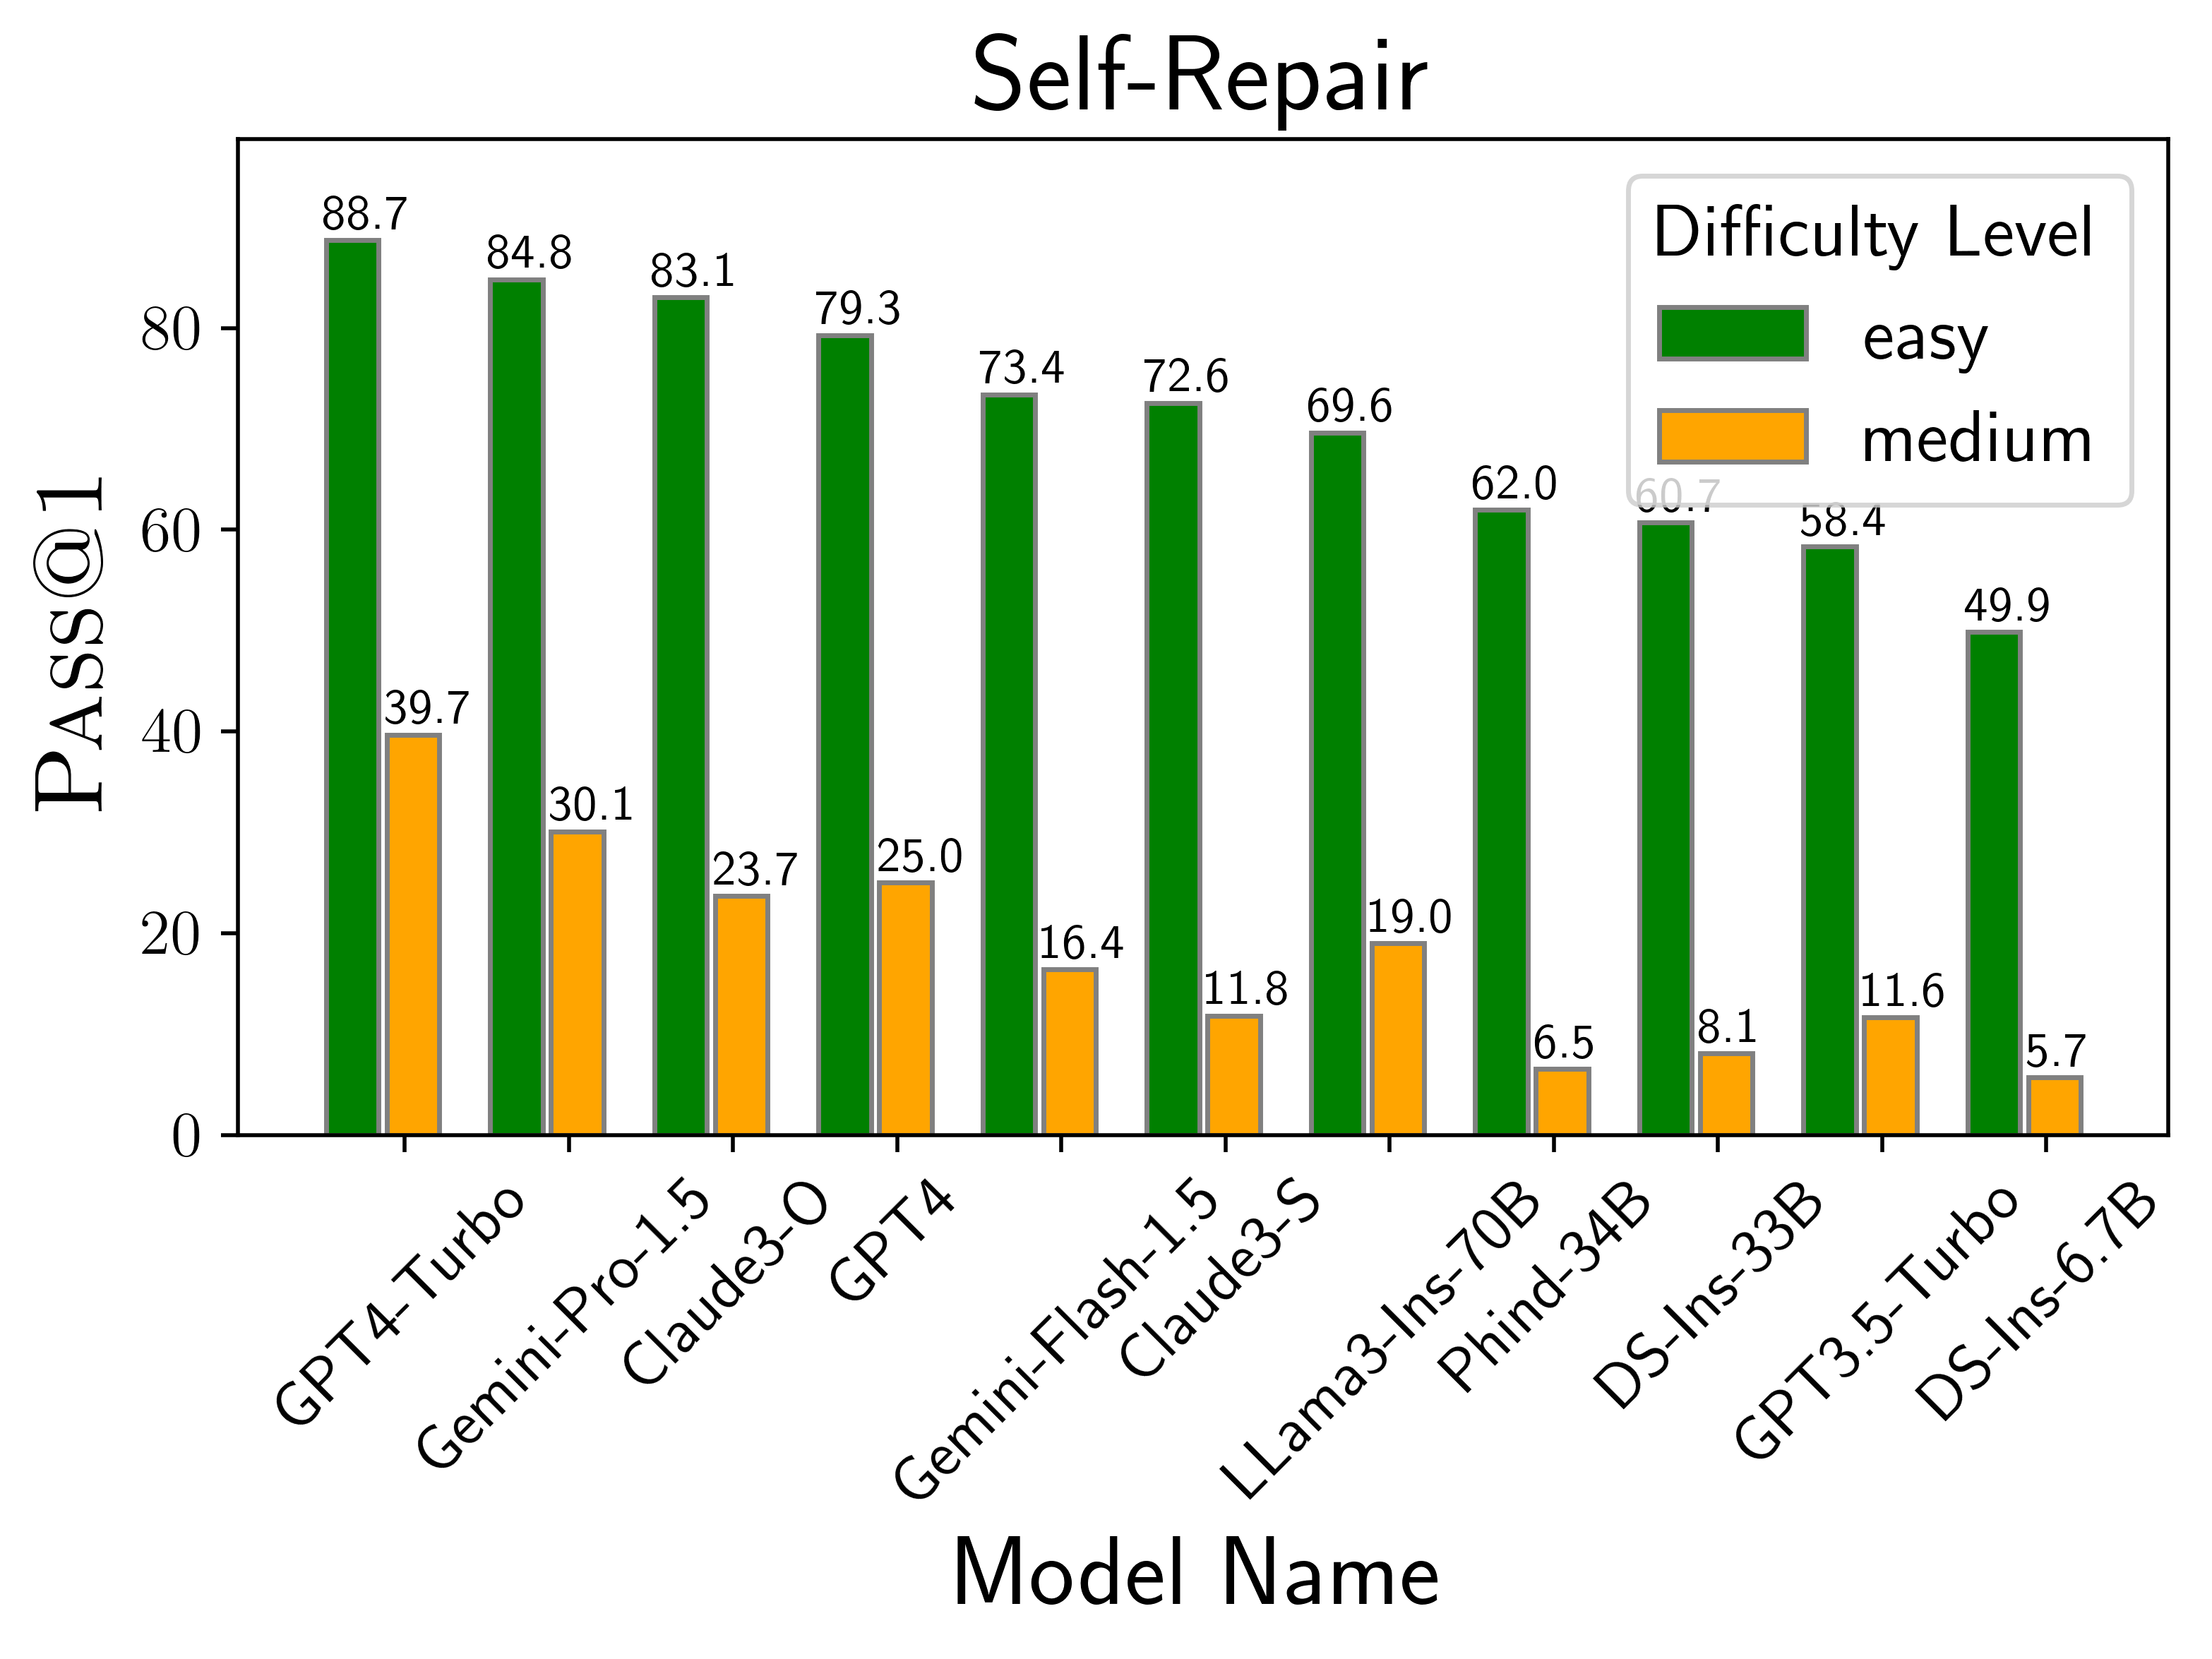
\includegraphics[width=0.48\linewidth]{figures/main_results/repair_performance.png}}
      
      \subfloat{
          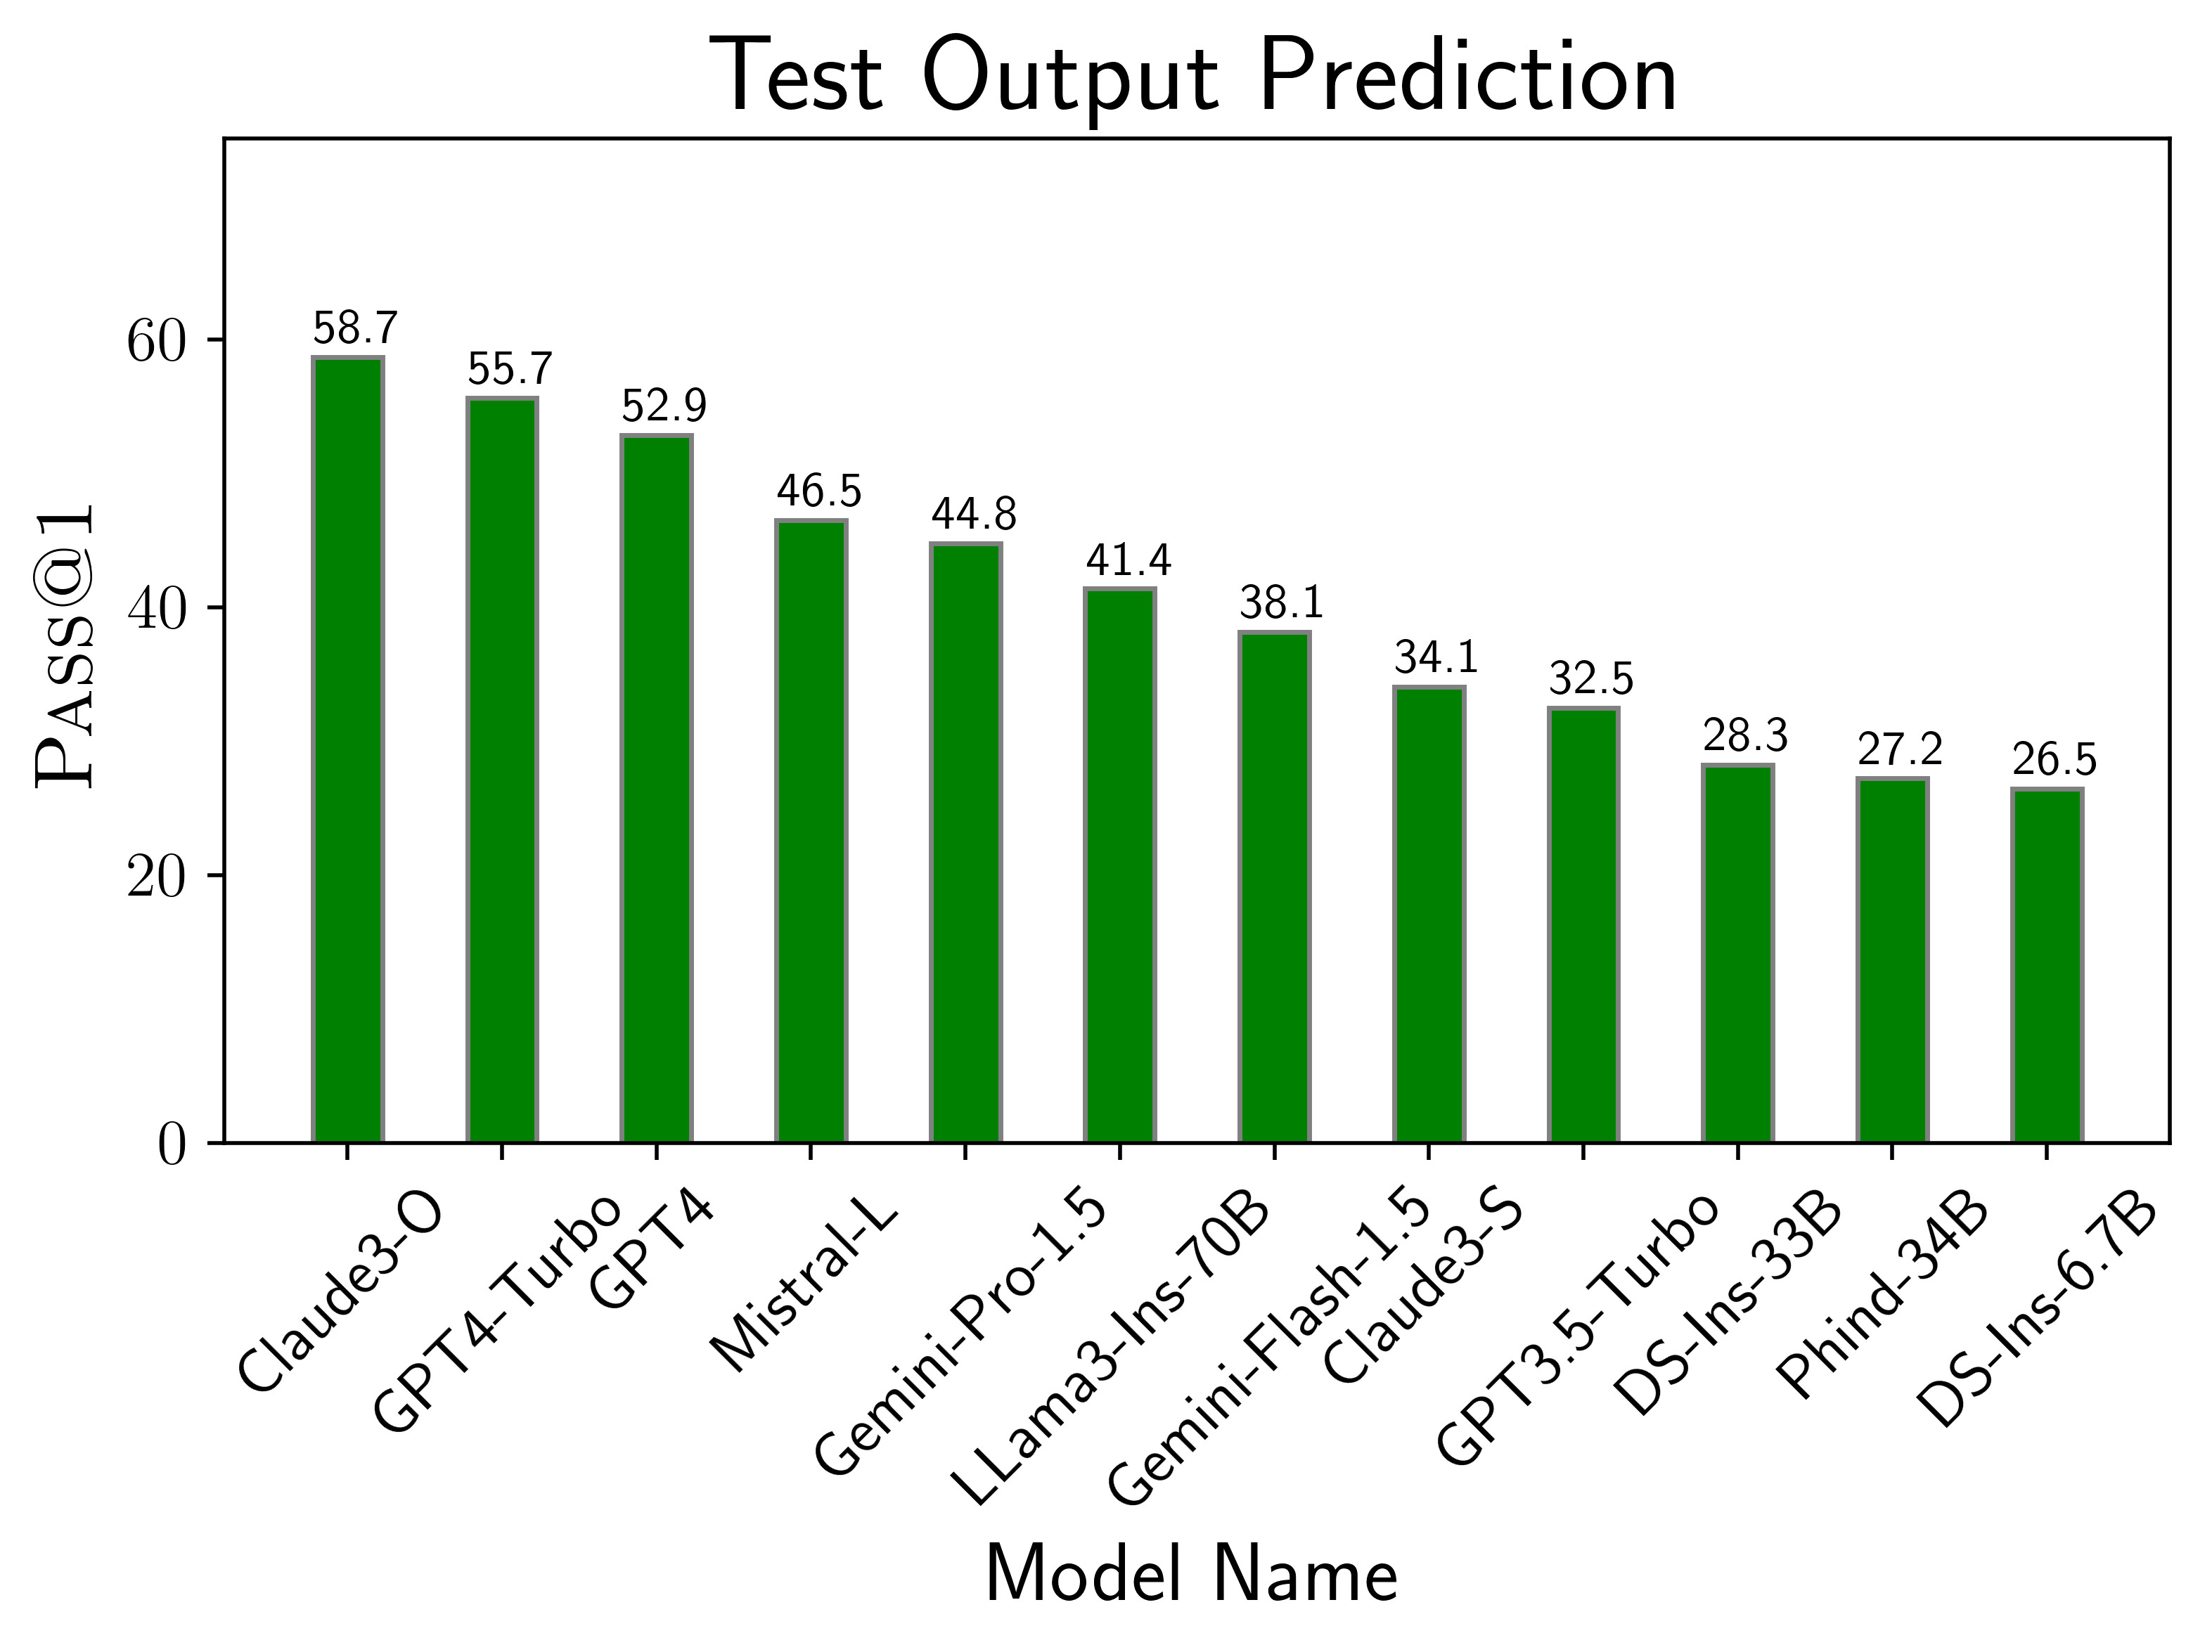
\includegraphics[width=0.48\linewidth]{figures/main_results/testgen_performance.png}}
      ~
      \subfloat{
        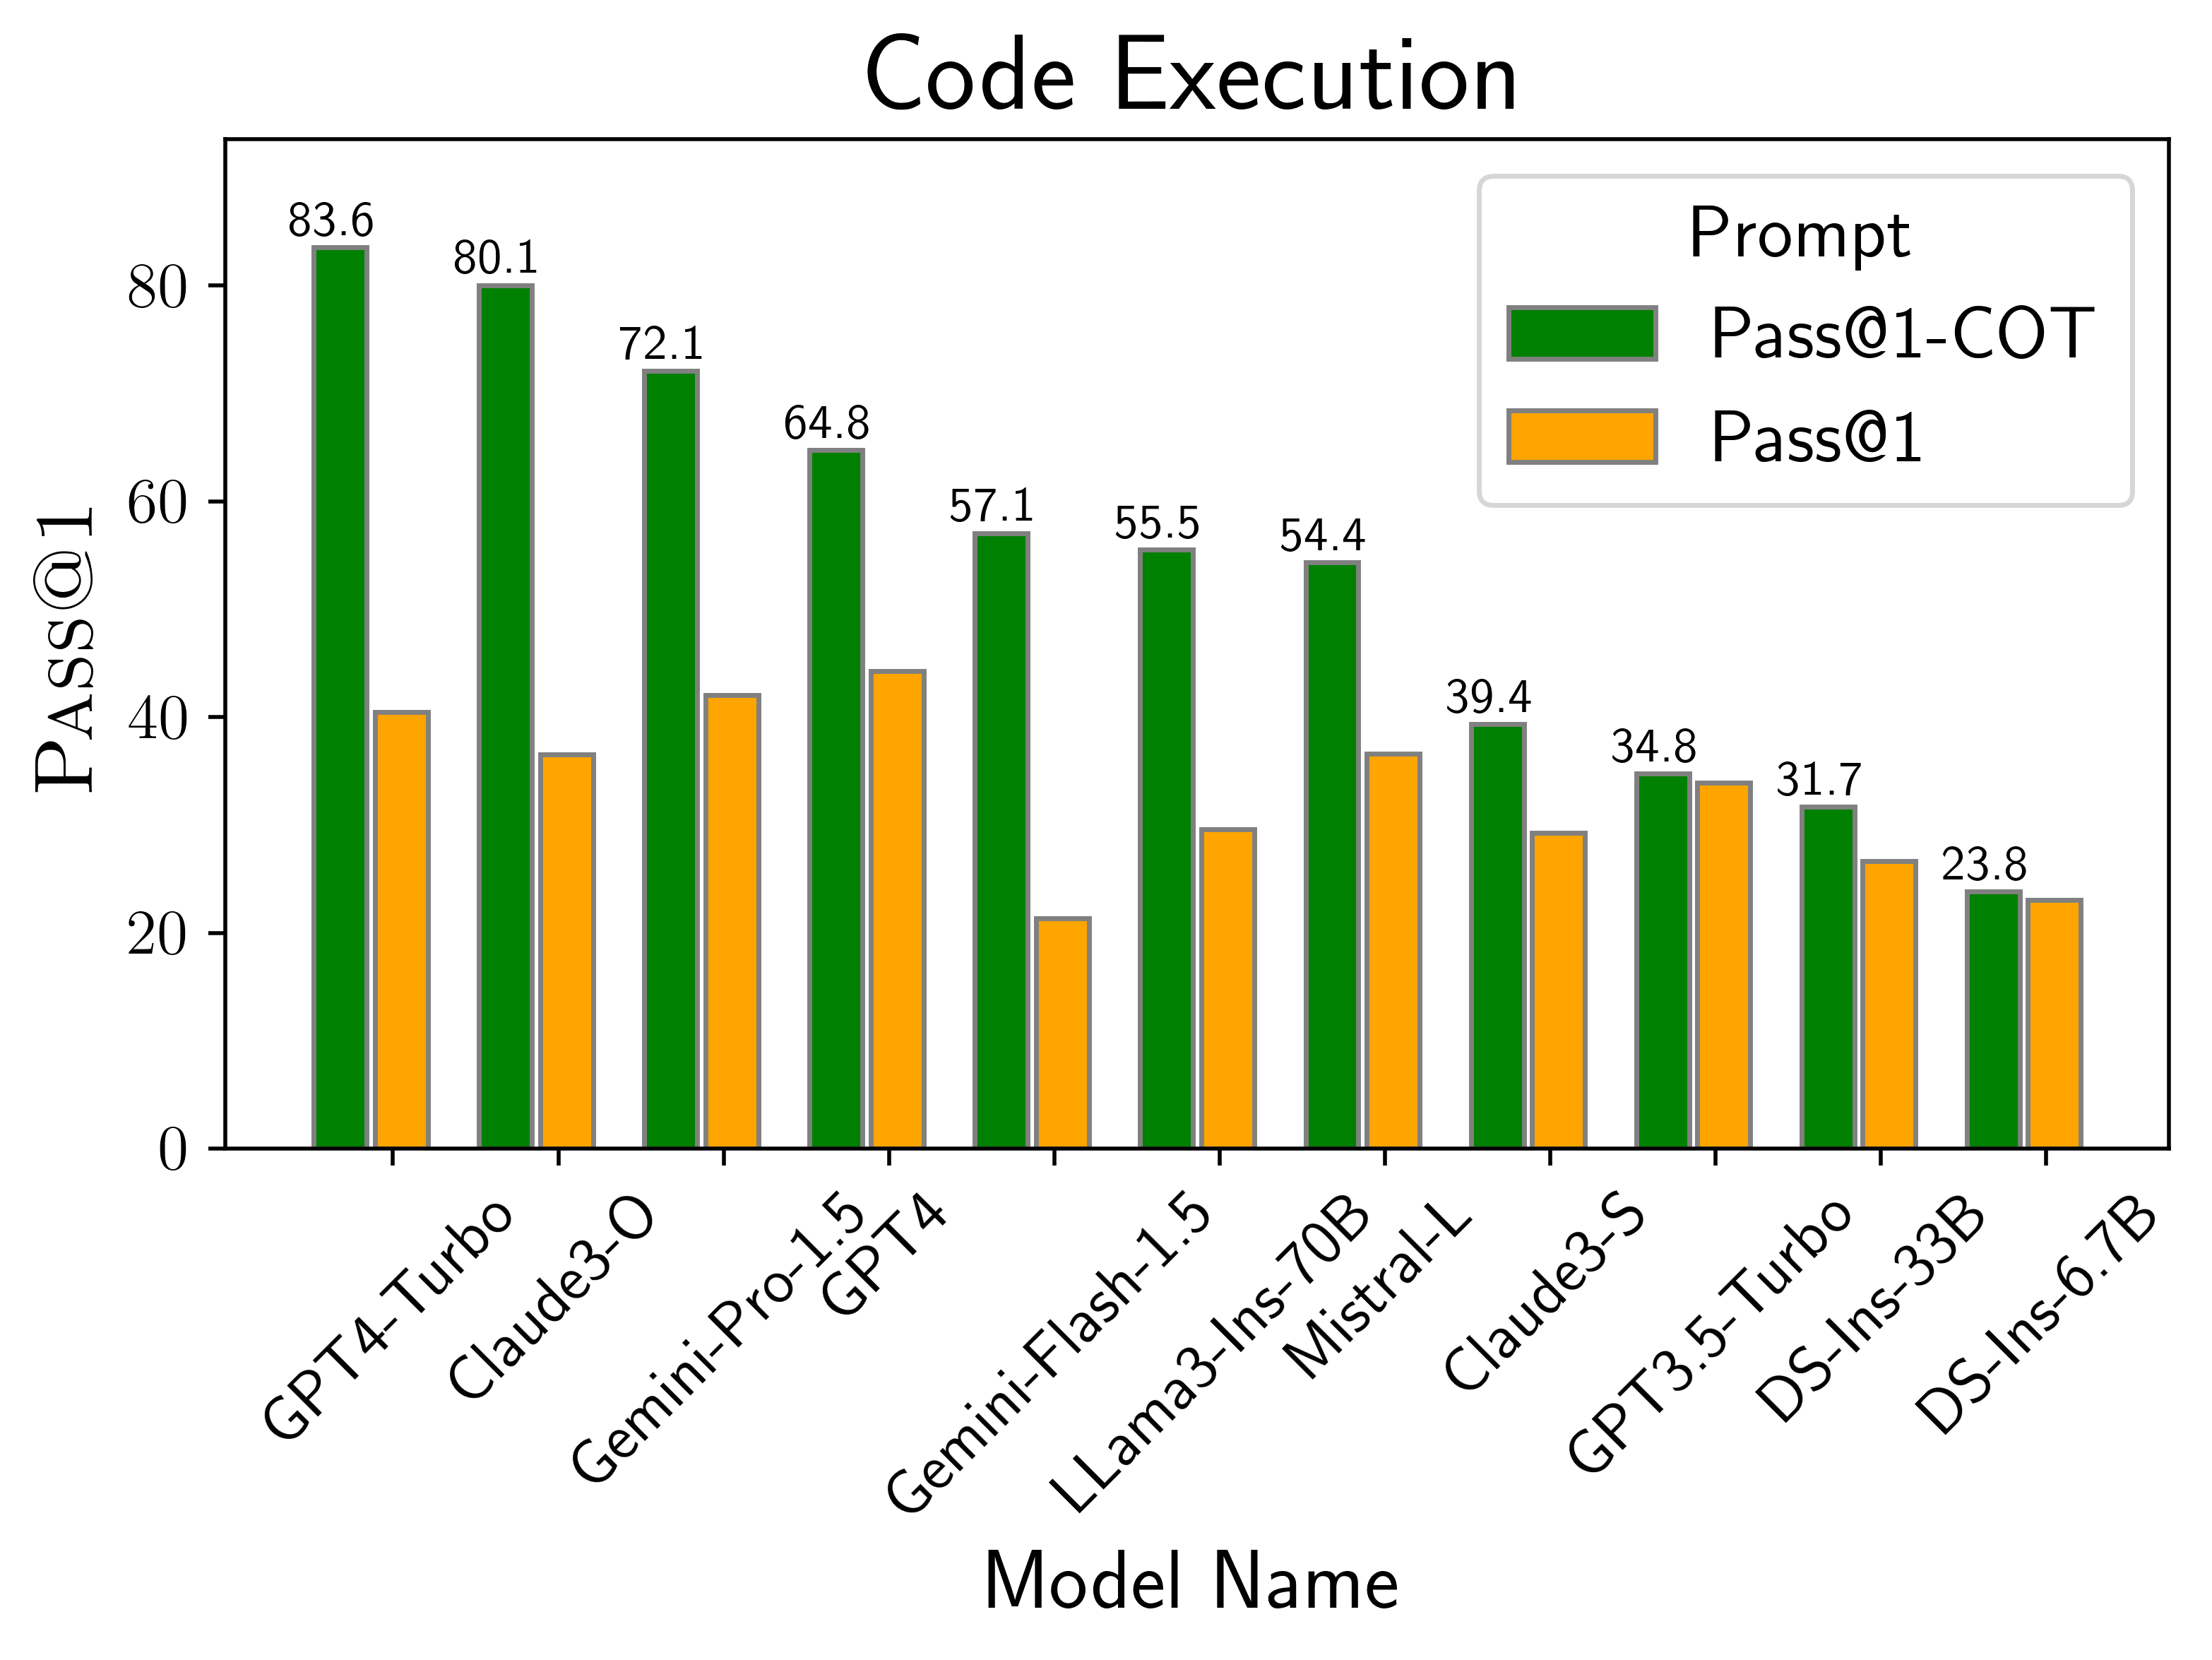
\includegraphics[width=0.48\linewidth]{figures/main_results/execution_performance.png}}
  
          %    ~
  %    \subfloat{
  %        \includegraphics[width=0.24\linewidth]{images/BB_CLASS/sensit-combined_valid_0.75.png}}
  \vspace{-5pt}
  \caption{
    Model performances across the four scenarios available in \livecodebench{}
    %(filtering on the time-window post September)
    .
    % The top-left and top-right plots depict \passmetric{1} of models on easy and medium splits across the code generation and self-repair scenarios respectively (results on hard subset deferred to the Appendix).
    %Performance of various models studied across different \livecodebench{} scenarios. 
    % The bottom-left and bottom-right plots depict \passmetric{1} of models across the test output prediction and code execution scenarios respectively.
  }
  \vspace{-16pt}
  
  \label{fig:results_plots}
  \end{figure*}
  

